
\chapter{Results}\label{cpt:Results}

%\section{System size impact on trophic levels}
%https://en.wikipedia.org/wiki/Trophic_level
%Snyggt att landskapet funkar och möjligen blir det lättare för detritusätarna att klara sig. Det slår mig att högre trofiska nivåer, som detritusätare, lider av en konversionsfaktor i energi: det måste finnas färre av dem. Finns det färre av dem är de mer utsatta för fluktuationer. Större system borde förbättra detta.
%\tempText{
%Energy conversion factor affecting detritus eaters? Try five different system sizes and investigate at what size detritus eaters can be sustained and if any organisms of even higher trophic levels emerge at larger system sizes.
%}
%\section{Influence of different habitats on emerging population}
%\tempText{Run simulations for equal time and parameter setup but one with terrain, one without, one in air, one in water, one in both.}
%\section{Large timescale simulation}\label{sec:largeTimescaleSim}
These results originate from a simulation run for 2 weeks, investigating the features emerging after long-term evolution in a large system. Many previous simulations had been performed with smaller world sizes, but while they achieved a larger number of total timesteps they did not contain the diversity and the trophic levels that resulted from this larger simulation. While it still remains a subject for further investigation, it at least seems as if a certain amount of organisms are needed on a trophic level before organisms on the next can be sustained.

\begin{table}[H]
 \begin{tabular}{| c || c | c | c|} 
    \hline
     Parameter &  Value \\ [0.5ex] 
     \hline\hline
     World size & \(350 \times 150 \times 350\) \\ \hline
     Timestep length & 0.01s \\ \hline
     Timesteps simulated & 1\,160\,000 \\ \hline
     Simulated time & 3h, 46m, 20s \\ \hline
     Simulation runtime & 14 days, 2h, 46m \\ \hline
 \end{tabular}
\caption{Statistics about the performed large timescale simulation, detailing its extent and magnitude}
\label{tab:longRunParameters}
\end{table}

\section{Initial organism}\label{sec:initOrg}
The initial organism was designed such that it would have a very simple genome and a non-existent nervous system, but so that it would still be able to survive long enough to reproduce. As can be seen in Figure \ref{fig:initOrg}, the inputs to the genome network comes from the input node 1, \(n_1\), and the bias node 15, \(n_{15}\). The interpretation of all node indices can be found in Subsection \ref{subsec:genToPhenMapping}.

While the bias node gives a constant signal of 1, the input \(n_1\) follows the value of the y-coordinate. The output node \(n_4\) corresponds to the photosynthetic cell type while \(n_{10}\) corresponds to egg cells and \(n_{13}\) does nothing. The connection to \(n_{13}\), as well as the node itself, is a residue left by mistake from earlier versions of a model where more properties were determined by the genome.

\begin{figure}
  \begin{center}
  \includegraphics[width=0.5\textwidth]{"figure/org0 genome"}
  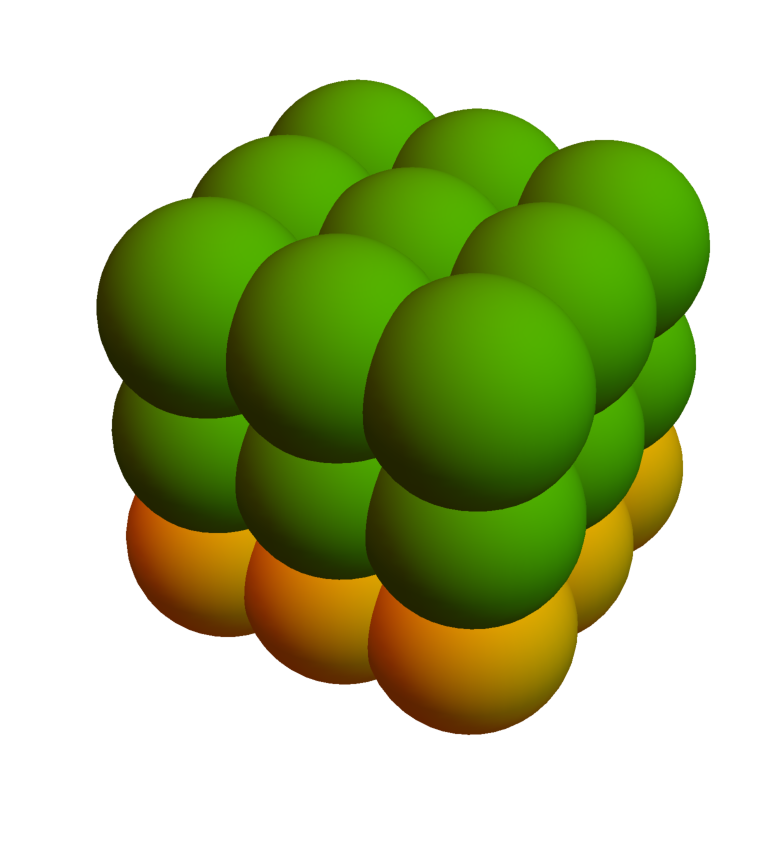
\includegraphics[width=0.3\textwidth]{figure/org0}
  \caption{
    Initial organism genome and visualisation. No hidden nodes exists in the network. Since the nervous system had no initial connections, the organism was inanimate and hence no nervous system network is displayed here.  
  }
  \label{fig:initOrg}
  \end{center}
\end{figure}

\section{Lineages and trophic levels}
Since there is no sexual reproduction within a model the notion of species cannot really be applied, however it is possible to follow and compare differently adapted ancestral lines. The clearly dominant type of organism belongs to the plant-like line exemplified in Figure \ref{fig:increasingSize}, but the results also include organisms of higher trophic levels resembling the adaptions of decomposers and plant-eating animals (herein called predators).

\subsection{Plants}
Plants are organisms that gain energy through their photosynthetic cells. Looking at figure \ref{fig:cellTypesOverTime} it is clear that a large majority of the cells (over 90 percent) are photosynthetic, something that is also supported by the green cover of vegetation seen in figure \ref{fig:arenaAtEnd}. Since the photosynthetic surface-dwellers are a large majority of the total population, the conclusions drawn here will mostly be taken from an analysis of the whole population average. This subsection will cover a number of the adaptions to be found in the photosynthetic organisms.

\begin{figure}
  \begin{center}
  \includegraphics[width=\textwidth]{figure/arenaAtEnd}
  \caption{Simulation arena at the end of the simulation, at t=1\,160\,000. While the organisms have spread all over the arena, the large majority is found on the surface level.}
  \label{fig:arenaAtEnd}
  \end{center}
\end{figure}

\begin{figure}
  \begin{center}
  \includegraphics[width=\textwidth]{figure/cellTypesOverTime}
  \caption{Number of cells belonging to each respective cell type over time. Note that the y-axis is logarithmic and that the photosynthetic cells thus represents a large majority. At the final timestep t=1\,160\,000 the photosynthetic cells constitutes 90.83\% of the cells, while the digest and sting cells are at 6.45\% and 0.23\% respectively. Vascular, fat, sense and buoyancy cells, having no part in energy collection or reproduction are very uncommon.}
  \label{fig:cellTypesOverTime}
  \end{center}
\end{figure}

\subsubsection{Swimming upwards}
One of the first mutations that shows signs of adaption is the upwards movement. There were mutations involving buoyancy cells that allowed very early organisms to float to the surface, but since those cells either replaced the photosynthetic cells or the egg cells those organisms were short-lived. After some sideways-moving organisms had started to spread across the water and, later on, some ventured a little higher, the organisms finally started inhabiting the surfaces at around t=130\,000. At t=200\,000, a population dense with organisms started out in the small lagoon at the corner of the map and soon the entire surface of the water was covered, as can be seen in Figure \ref{fig:altidudeDensity}.
\begin{figure}
  \begin{center}
  \includegraphics[width=0.7\textwidth]{figure/altitudeDensity}
  \caption{
    Cell altitude density over time. The more cells that occupy a given altitude (y-coordinate) at a given timestep, the more light the point appear in the chart. The plot range is clipped at a cell density of 5000, but the lightest area reaches close to 40\,000 at around t=600\,000. Due to gravity, the initial organism, having spawned in the exact centre of the arena, quickly falls to the bottom, below the water surface. This is where the population starts out, at an altitude of about 30, which can be seen in the bottom-left corner of the chart. Quite quickly however, the organisms evolve movement vectors upwards and the large majority end up at the altitude of 75 by the water surface, after about t=200\,000.
    The fact that the organisms are spread out and focused on different altitudes shows signs of niche adaption.
  }
  \label{fig:altidudeDensity}
  \end{center}
\end{figure}

\subsubsection{Larger organisms}
Another trend for the organisms is that they increase in size. Looking at the charts in Figure \ref{fig:nOrgs} it is clear that the population increased exponentially until about t=300\,000 after which the number of cells remained approximately constant while the number of organisms steadily decreased. The bottom chart shows even clearer how the size of the organisms then started to increase. The time t=300\,000 is also right after the water surface got crowded with photosynthetic organisms. A probable explanation for the increase in size is therefore that it is an adaption resulting from the competition for the water surface area; a larger more spread-out organism can harvest more energy and reproduce faster. This is supported by observation of the surface organisms getting increasingly spread-out over the generations.
\begin{figure}
  \begin{center}
  \includegraphics[width=0.60\textwidth]{figure/particles}
  
  \vspace{0.5cm}
  
  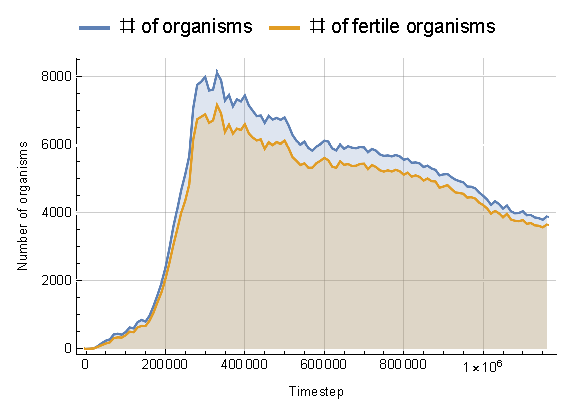
\includegraphics[width=0.60\textwidth]{figure/nOrgs}
  
  \vspace{0.5cm}
  
  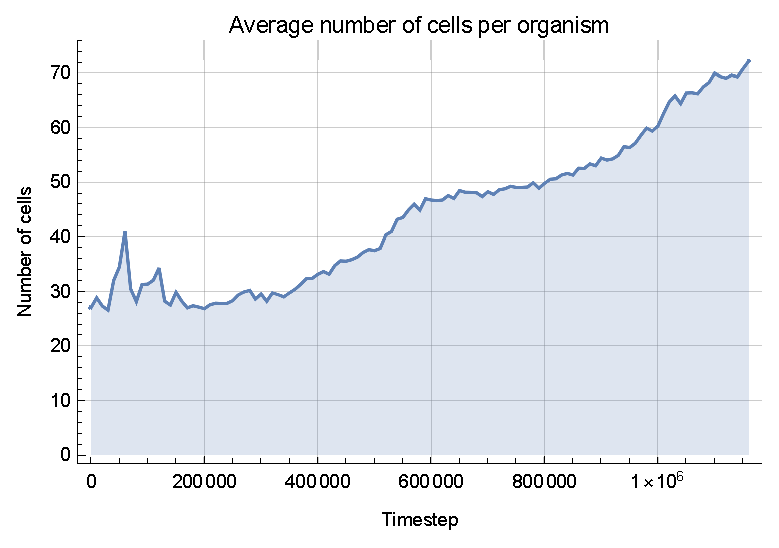
\includegraphics[width=0.60\textwidth]{figure/nCells}
  \caption{
  Simulation statistics over time. As can be seen in the top-left chart, the number of particles stabilised after around t=300\,000. However, the number of organisms (top-right chart) henceforth decreased steadily. This can be explained by the bottom chart, which clearly shows that the size of the organisms has, on average, increased over time. The jumps in the number of buffer particles is only the model ensuring that there are enough buffer particles available.
  }
  \label{fig:nOrgs}
  \end{center}
\end{figure}

\tempText{
Note about Cope's rule and possible validity? \url{https://en.wikipedia.org/wiki/Cope's_rule}
}

\begin{figure}
  \begin{center}
  \includegraphics[width=\textwidth]{figure/increasingSize}
  \caption{
  Example of morphology changing over time. Phenotype for every tenth ancestor of the organism with index 574174, which was one of the organisms living on the water surface at t=1\,000\,000. It is located in the top-left corner, the oldest ancestor is in the bottom-right, as indicated by the generation labels. A trend of this ancestral line is that the organisms have increased in size, as well as turning more "pyramid-shaped". The radius of the top cells are, in the later organisms, significantly smaller than the bottom cells.
  }
  \label{fig:increasingSize}
  \end{center}
\end{figure}

\subsubsection{Pyramid-shaped organisms}
Apart from increasing in size, the water-surface organisms also became more "pyramid-shaped" over time, as seen in Figure \ref{fig:increasingSize}. This enables the lower layers of the organism to extract photosynthetic energy as well, instead of relying on the energy from the top layer like their early ancestors. It is interesting to note that this is a direct artefact from how the model was implemented, with the energy-particles checking for occluding particles above as described in \ref{sec:EnergyCycle}

\subsubsection{Higher ratio of fertile organisms}
Observing the top-right chart of Figure \ref{fig:nOrgs} it looks as if the proportion of organisms that are fertile (meaning that they have at least one egg cell) are increasing relative to the total number of organisms over time. This is even more evident in Figure \ref{fig:fertileProp} where, after an initial drop from unity caused by the single initial organism and it's immediate offspring, the proportion steadily approaches a level of almost \(0.95\).

A certain proportion of the organisms could be expected to not be fertile, since there is always a certain non-zero probability for each offspring to be born without egg cells. Since non-fertile organisms per definition cannot produce offspring it is clear to see that their proportion should not increase. However, the fact that the fertile proportion is steadily increasing, instead of remaining constant, seem to show an emerging resilience in the genome against birthing non-fertile offspring.

A majority of all the organisms that ever existed in the simulation never did reproduce, as can be seen in Figure \ref{fig:numberOfChildren}. Some of those were not fertile while most simply died before they had gathered enough energy in their egg cells. Out of those that did reproduce, most had between one and two children, but close to 15 percent of the organisms had more than two children, with one having as many as 27.

\begin{figure}
  \begin{center}
  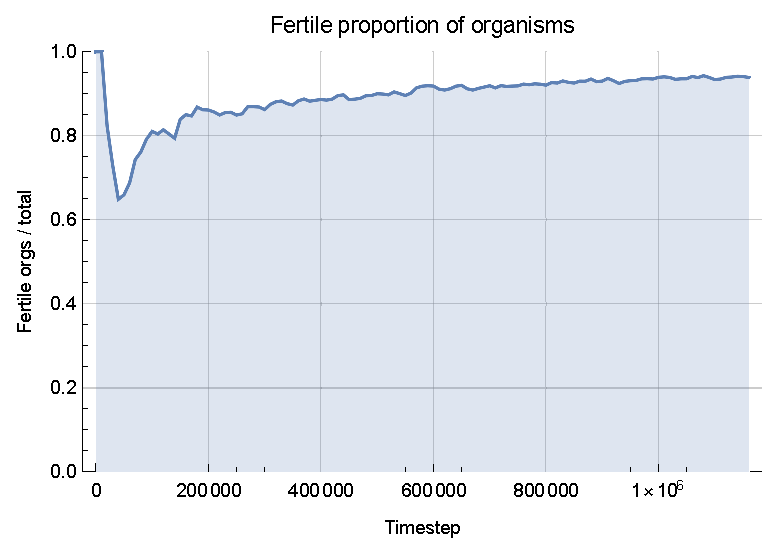
\includegraphics[width=0.6\textwidth]{figure/fertileProp}
  \caption{
    Number of fertile organisms divided by the total number of organisms over time.
  }
  \label{fig:fertileProp}
  \end{center}
\end{figure}

\begin{figure}
  \begin{center}
  
  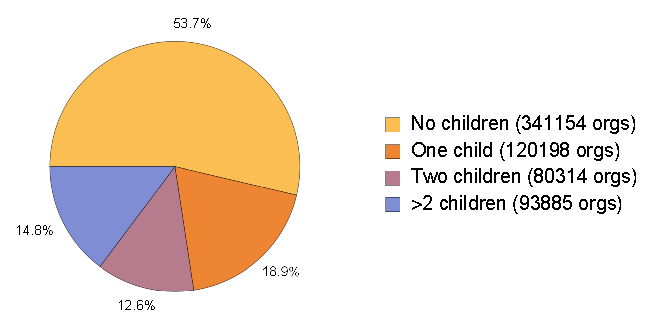
\includegraphics[width=0.6\textwidth]{figure/nChildrenPie}
  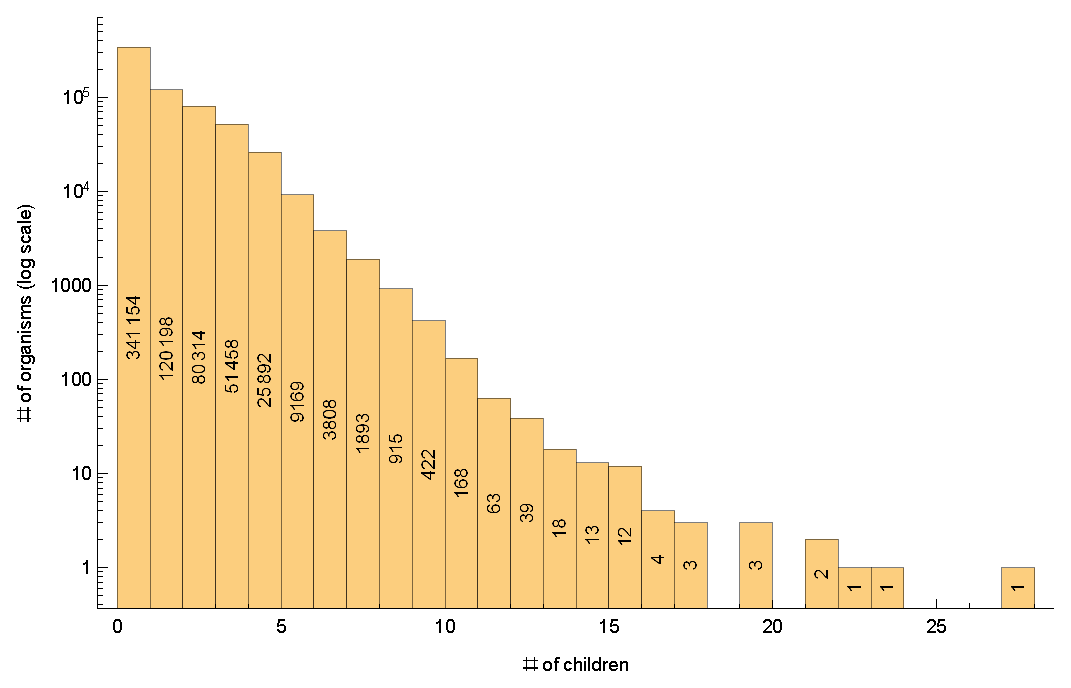
\includegraphics[width=0.8\textwidth]{figure/nChildrenHistogram}
  \caption{
    Distribution of number of children per organism, given all organisms throughout the whole simulation. A majority of the organisms never reproduced but multiple children are not uncommon among those that did, as can be seen in the histogram on the bottom. Note that the y-axis is logarithmic and that the amount of children as such follows a power-law distribution.
  }
  \label{fig:numberOfChildren}
  \end{center}
\end{figure}

\subsubsection{Fewer eggs per organism}
A clear adaption is the fact that the average number of egg cells per organism has dropped. The initial organism had a total of nine egg cells, resulting merely from the fact that it allowed the genome to stay simple while still allowing the organisms to reproduce. That many egg cells were however redundant and the population eventually evolved to settle on the lower value of two eggs per organism, as can be clearly seen on Figure \ref{fig:nEggs}. 

\begin{figure}
  \begin{center}
  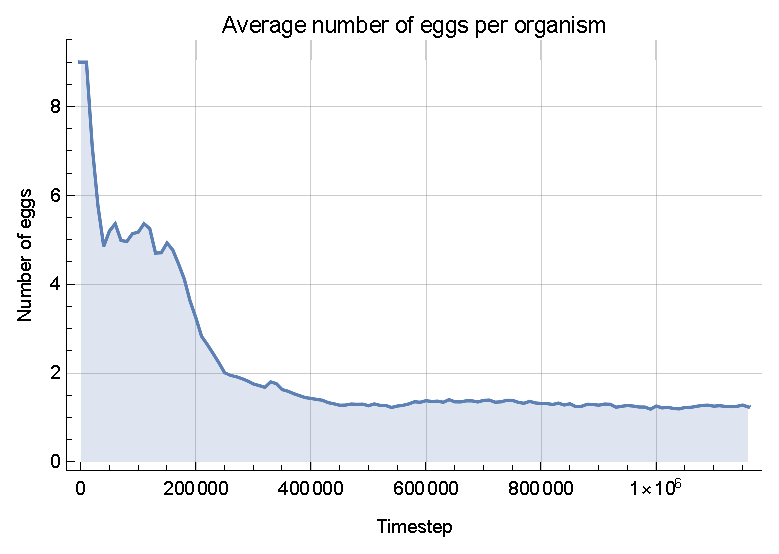
\includegraphics[width=0.6\textwidth]{figure/nEggs}
  \caption{
    The average number of egg cells per organism over time. At about the same time as the total number of cells in the simulation stabilised (t=400\,000) each organism settled on having about one egg cell each.
  }
  \label{fig:nEggs}
  \end{center}
\end{figure}

\subsubsection{Three plant organisms}\label{subsubsec:3plants}
Table \ref{tab:3plants} shows a selection of three different plants and their properties. Noting the position of \emph{plantA}, its altitude (y-coordinate) of just above 100 places it a bit above the water surface of 75. Studying the x and z coordinates it can be determined that it is located upon the terrain, up on dry land. Comparing this with \emph{plantB}, which position places it directly at the water surface, it is clear that while both plants have adapted in size and shape for efficient photosynthesis, their separate environments have caused them to evolve in parallel. As seen in Figure \ref{fig:familyTree}, the most recent common ancestor of \emph{plantA} and \emph{plantB} is at generation 61, while \emph{plantB} and \emph{plantC} share a more recent ancestor at generation 96. The closer relationiship between \emph{plantB} and \emph{plantC} can also be seen in their more similar morphology. However, \emph{plantC} has a much higher y-coordinate, placing it floating in the air far above the surface and very close to the top of the arena at 150. While this height altitude is beneficial in that it ensures a clear view for photosynthesis, it also costs more energy to keep afloat in the low-density air. 

The third column of the table, \emph{plantC}, shows a plant organism that resides in the air, far above the surface and close to the top of the arena.
\begin{table}[H]
 \begin{tabular}{ c || c | c | c |} 
    & plantA & plantB & plantC \\ [0.5ex] \hline \hline
     Organism ID & 634078 & 574174 & 628131 \\ \hline
     Generation & 148 & 121 & 136 \\ \hline
     Timestep of birth & 1157422 & 999961 & 1140031 \\ \hline
     Timestep of death & (still alive) & 1000654 & 1160034 \\ \hline
     Visualisation & 
        \includegraphics[width=0.2\textwidth]{figure/3orgs/plantA} &
        \includegraphics[width=0.2\textwidth]{figure/3orgs/plantB} &
        \includegraphics[width=0.2\textwidth]{figure/3orgs/plantC} \\
     (at timestep) & 1150000 & 1140000 & 1130000 \\ \hline
     Position \(\left(\begin{array}{l} x\\y\\z\end{array}\right)\) & 
        \(\left(\begin{array}{l} 172.198\\101.756\\74.0961 \end{array}\right)\) &
        \(\left(\begin{array}{l} 108.528\\ 74.7777\\ 341.747\end{array}\right)\) &
        \(\left(\begin{array}{l} 39.015\\ 149.276\\ 254.073\end{array}\right)\)\\ \hline
 \end{tabular}
\caption{Example of three different plant organisms, each using photosynthesis but occupying different parts of the arena and having different adaptions.}
\label{tab:3plants}
\end{table}

\subsection{Decomposers}
Decomposers gain energy through their digestive cells, eating detritus particles as they fall down from dying organisms above. Differing from the plants, the decomposers have maintained the dimensions of the initial organism. Being significantly fewer, there is not the same need to compete for space.

The decomposers are mostly made up of digestive cells and a single egg cell, although some decomposing lineages contain other cell types as well. Some, like \emph{decompA} in Table \ref{tab:3decomp}, has a single (or a few) photosynthetic cells, perhaps useful if they ever get a clear view of the sky, but maybe just a relic from previous generations. There is also a lineage that has a single or multiple vascular cell adjacent to their egg cell, an example of this is \emph{decompB} in Table \ref{tab:3decomp}. This might be an adaption to better transport the energy from digestive cells to the egg cell, like the vascular cell was intended.

\begin{figure}
  \begin{center}
  \includegraphics[width=\textwidth]{figure/vascularDecomposers}
  \caption{Rendered view of decomposers living off eating the dead cells falling down from the surface-level plants. Note the occasional light-blue vascular cell in some of the decomposers.}
  \label{fig:vascularDecomposers}
  \end{center}
\end{figure}

\subsubsection{Three decomposer organisms}\label{subsubsec:3decomp}
As can be seen in Table \ref{tab:3decomp}, three decomposer organisms have been selected as examples of their lineages. As discussed above, they contain mostly digestive cells, a single egg cell and, in the first two organisms, cells of other types. The positions of the decomposer organisms are closer together than those of the plant organisms (as can be seen in Figure \ref{fig:lineOrgPos}), explained by the fact that decomposers occupy a single niche at the bottom below the water surface.
\begin{table}[H]
 \begin{tabular}{ c || c | c | c |} 
    & decompA & decompB & decompC \\ [0.5ex] \hline \hline
     Organism ID & 634597 & 634413 & 634596 \\ \hline
     Generation & 220 & 234 & 206 \\ \hline
     Timestep of birth & 1158806 & 1158364 & 1158806 \\ \hline
     Timestep of death & (still alive) & (still alive) & (still alive) \\ \hline
     Visualisation & 
        \includegraphics[width=0.2\textwidth]{figure/3orgs/decompA} &
        \includegraphics[width=0.2\textwidth]{figure/3orgs/decompB} &
        \includegraphics[width=0.2\textwidth]{figure/3orgs/decompC} \\
     (at timestep) & 1160000 & 1160000 & 1160000 \\ \hline
     Position \(\left(\begin{array}{l} x\\y\\z\end{array}\right)\) & 
        \(\left(\begin{array}{l} 102.983\\45.5508\\198.9 \end{array}\right)\) &
        \(\left(\begin{array}{l} 107.391\\52.922\\143.383\end{array}\right)\) &
        \(\left(\begin{array}{l} 128.907\\45.5792\\184.384\end{array}\right)\)\\ \hline
 \end{tabular}
\caption{Example of three different decomposer organisms, each gaining energy from eating detritus particles}
\label{tab:3decomp}
\end{table}

\subsection{Predators}
The adapted line called predators is characterised by their use of sting cells to steal energy from the living cells of other organisms. They are however similar to decomposers in that they also have digestive cells, utilised when their prey dies or when no living organisms can be found.

Compared to plants and decomposers, which as a rule tend to have one egg cell per organism, the predators have a lot more. This adaption can be explained by the fact that predators gain their energy at non-regular intervals; sting cells only gain energy while in contact with living cells from other organisms and there are not always other organsism present. When they do gain energy however, it could very well be more than what fits in a single egg cell and so multiple egg cells ensures that no energy goes to waste. This also explains the fact that Figure \ref{fig:nEggs} approaches a value slightly above, but not equal to, one.

Figure \ref{fig:predLineage} shows an example of a predator lineage.

\begin{figure}
    \begin{center}
        \makebox[\textwidth]{\includegraphics[width=\textwidth]{figure/predLineage}}
    \end{center}
    \caption{
    Example of a predator lineage. Phenotype for every tenth ancestor of the organism with index 630807, which was one of the organisms living in the predator bay at the end of the simulation, at t=1\,160\,000. Note that the organism portraits are taken at certain exported frames and that, as such, some cannot be found while others have lost cells since their birth. The predators originate, as all organisms do, from the initial organism at generation 0.
    }
    \label{fig:predLineage}
\end{figure}

\subsubsection{Three predator organisms}\label{subsubsec:3pred}
Compared to the three example organisms from the plant and decomposer lineages, the predator organisms are even more geographically constricted, as can be seen in Figure \ref{fig:lineOrgPos}. Looking at Table \ref{tab:3pred}, the predator organisms are also quite similar in their morphology; \emph{predA} and \emph{predC} are almost identical and while \emph{predB} has a larger ratio of sting cells, its original form of \(3 \times 3 \times 3\) cells has changed since its conception. The similarity between the organisms is not strange given their relatively recent common ancestor just a few generations earlier, as seen in Figure \ref{fig:familyTree}.
\begin{table}[H]
 \begin{tabular}{ c || c | c | c |} 
    & predA & predB & predC \\ [0.5ex] \hline \hline
     Organism ID & 630807 & 634099 & 634960 \\ \hline
     Generation & 255 & 255 & 255 \\ \hline
     Timestep of birth & 1148044 & 1157463 & 1159725 \\ \hline
     Timestep of death & (still alive) & (still alive) & (still alive) \\ \hline
     Visualisation & 
        \includegraphics[width=0.2\textwidth]{figure/3orgs/predA} &
        \includegraphics[width=0.2\textwidth]{figure/3orgs/predB} &
        \includegraphics[width=0.2\textwidth]{figure/3orgs/predC} \\
     (at timestep) & 1150000 & 1150000 & 1160000 \\ \hline
     Position \(\left(\begin{array}{l} x\\y\\z\end{array}\right)\) & 
        \(\left(\begin{array}{l} 318.756\\73.1252\\46.4154 \end{array}\right)\) &
        \(\left(\begin{array}{l} 330.843\\76.0001\\42.1454\end{array}\right)\) &
        \(\left(\begin{array}{l} 338.39\\74.9417\\40.7016\end{array}\right)\)\\ \hline
 \end{tabular}
\caption{Example of three different predator organisms, each gaining energy by stealing it from cells of other living organisms}
\label{tab:3pred}
\end{table}

\subsection{Inter-lineage relations}
From each lineage type, plants, decomposers and predators, three example organisms were chosen and investigated for their common ancestors. The resulting family tree is illustrated in figure \ref{fig:familyTree}. It can be seen already from the phenotype that similar organisms tend to be closer related. The plants and the predators actually share a more recent common ancestor compared to the decomposers, however since that plant is born very early, at generation 15, this should not hold much significance and can be mostly regarded as a result of the selected organisms.

\begin{figure}
  \begin{center}
  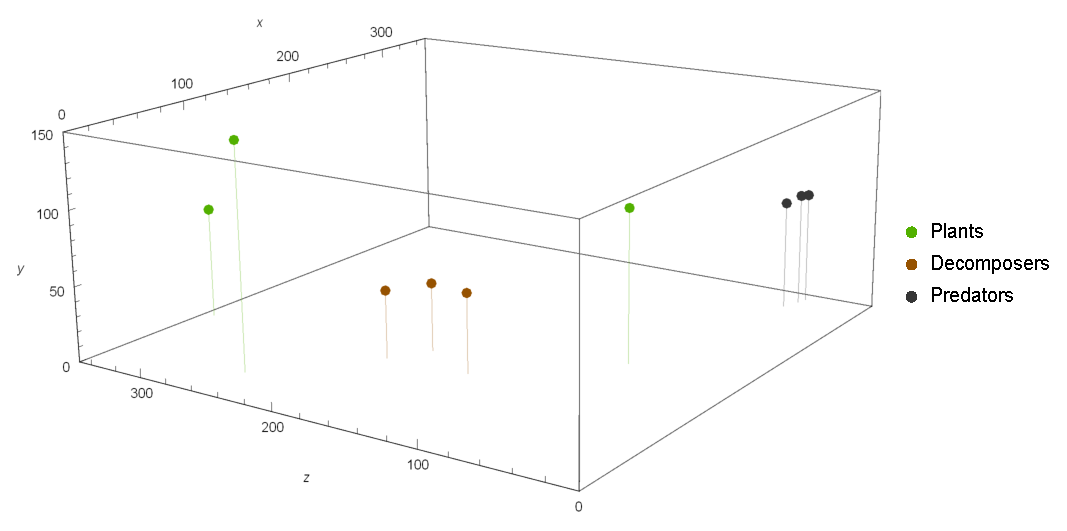
\includegraphics[width=0.9\textwidth]{figure/lineOrgPos}
  \caption{Positions of the nine example organisms described in subsections \ref{subsubsec:3plants}, \ref{subsubsec:3decomp} and \ref{subsubsec:3pred}}
  \label{fig:lineOrgPos}
  \end{center}
\end{figure}

\begin{figure}[ht]
    \begin{center}
        \makebox[\textwidth]{\includegraphics[width=\paperwidth]{figure/familyTree}}
    \end{center}
    \caption{
    Each of the the nine example organisms described in subsections \ref{subsubsec:3plants}, \ref{subsubsec:3decomp} and \ref{subsubsec:3pred} represent a lineage among either plants, decomposers or predators. This diagram represents them as the leaf nodes of their family three, with their mutual most common ancestors included, all the way to the initial organism. Note that the organism visualisations are taken from saved timesteps and that the organisms are at different stages of decay. The ancestor 624933 was not found on any saved timestep on record
    }
    \label{fig:familyTree}
\end{figure}
% Det roligaste vore ju om det gick att följa en någorlunda lång körning där det uppstår några adapterade linjer - arter blir det ju inte eftersom de inte fortplantar sig sexuellt. Då skulle du kunna avbilda dem och beskriva vad de gör och hur deras fenotyper verkar vara adapterade. Sen skulle du kunna följa dem bakåt för att se hur tidigare former ser ut, när dessa anpassningar uppstod och så vidare. Sen skulle du kunna plocka ut en representant för varje sort och visa släktträdet. Hur såg den senaste gemensamma föregångaren till dem ut? Kanske displayat i ett träd. Hur har ekosystemet utvecklats? Har olika trofiska nivåer uppstått? Två nivåer har vi ju sett: sol och detritus - fattas då bara predatorer.

\section{Genomes over time}
Figure with increasing genome and nervous system sizes
\begin{figure}
  \begin{center}
  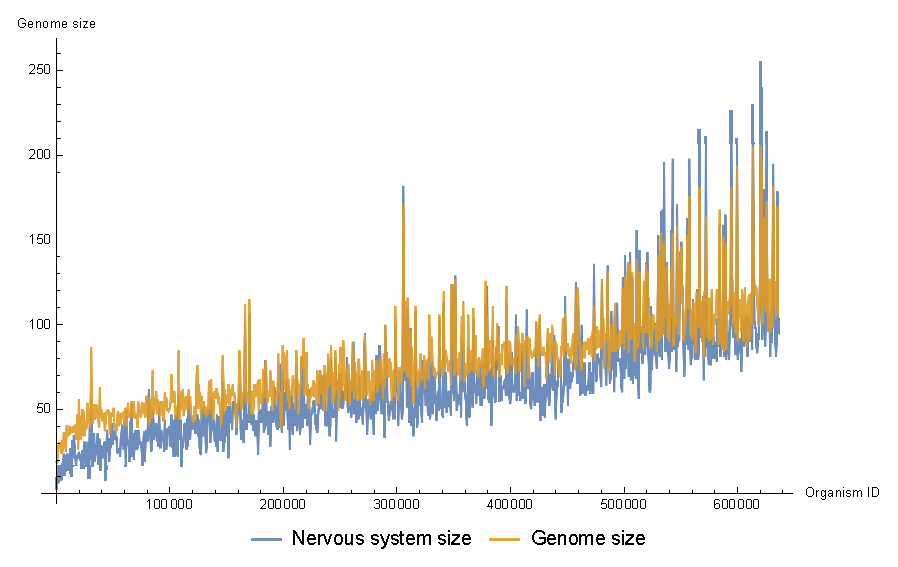
\includegraphics[width=0.7\textwidth]{figure/genomeSizes}
  \caption{
    Figure with increasing genome and nervous system sizes
  }
  \label{fig:genomeSizes}
  \end{center}
\end{figure}

\begin{figure}[ht]
    \begin{center}
        \makebox[\textwidth]{\includegraphics[width=0.9\paperwidth]{"figure/org574174 genome"}}
    \end{center}
    \caption{Genome (left) and nervous system (right) of the surface-dwelling plant with id 574174.}
    \label{fig:planGgenome}
\end{figure}

\tempText{Nodes filled with blue???}